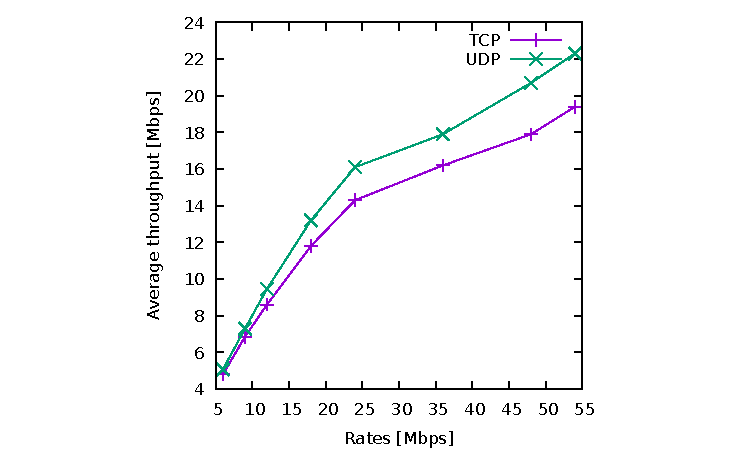
\includegraphics[width=0.5\textwidth]{traces/L3-1-4-tput.pdf}
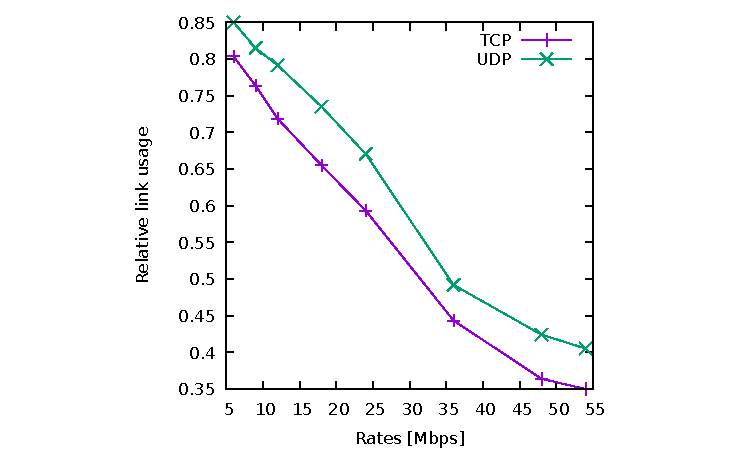
\includegraphics[width=0.5\textwidth]{traces/L3-1-4-usage.pdf}
UDP's throughput is consistenly higher than TCP's. TCP has larger headers so more overhead. More importantly, TCP's congestion control mechanisms lead to reduced throughput. TCP will occasionally not send as fast as the network could handle (mainly during slow start), while UDP is constantly transmitting as fast as the wnic will allow it to. Throughput grows together with bitrate: the network supports sending more bits per second with higher bitrates. \\ \\
The throughput does not grow as quickly as the bitrate: with higher bitrates the bits are sent faster and bits are more likely to get lost. For TCP this triggers retransmissions and congestion control. For UDP the lost data is simply not counted towards the throughput. Both have a negative effect on throughput. This means doubling the bitrate does not double the observed throughput. This translates to a decreasing usage with increasing bitrate.
